% Workspace Lenses at Small Scale -- arXiv preprint source.
% Build:  pdflatex main && bibtex main && pdflatex main && pdflatex main
% Every number in this file comes from a results file in ../../results (see Appendix A).
% Results that are still being computed are marked with \pending{...}; they render as red notes.

\documentclass[11pt]{article}

\usepackage[T1]{fontenc}
\usepackage[utf8]{inputenc}
\usepackage{lmodern}
\usepackage[margin=1in]{geometry}
\usepackage{microtype}
\usepackage{amsmath,amssymb,amsthm}
\usepackage{bm}
\usepackage{booktabs}
\usepackage{multirow}
\usepackage{graphicx}
\usepackage{caption}
\usepackage{xcolor}
\usepackage{enumitem}
\usepackage[numbers,sort&compress]{natbib}
\usepackage[colorlinks=true,linkcolor=blue!50!black,citecolor=blue!50!black,urlcolor=blue!50!black]{hyperref}
\usepackage{cleveref}

\captionsetup{font=small,labelfont=bf}
\setlist{nosep,leftmargin=*}

\newtheorem{proposition}{Proposition}
\newtheorem{corollary}{Corollary}
\newtheorem{observation}{Observation}
\theoremstyle{definition}
\newtheorem{definition}{Definition}

\newcommand{\pending}[1]{\textcolor{red!70!black}{\textbf{[Pending:} #1\textbf{]}}}
\newcommand{\E}{\mathbb{E}}
\newcommand{\R}{\mathbb{R}}
\newcommand{\Jl}{J_{\ell}}
\newcommand{\tr}{\operatorname{tr}}
\newcommand{\jpp}{J{+}{+}}

\title{Workspace Lenses at Small Scale:\\
Reproducing the Jacobian Lens and J++ on Qwen3-0.6B,\\
with Label-Free and Broadcast Variants}

\author{Author names withheld (draft)}
\date{November 2026}

\begin{document}
\maketitle

\begin{abstract}
The Jacobian lens (J-lens) reads an intermediate residual-stream vector of a language model through
the corpus-averaged Jacobian to the final layer, and the tokens it surfaces in a mid-depth band have
been argued to behave like the contents of a global workspace. The J++ lens makes these readouts
markedly more faithful in large models. We reproduce the J-lens, the R-Lens and J++ on Qwen3-0.6B
on a single CPU, using the released prompt sets and the J++ evaluation protocol, and ask which of the
workspace properties survive at sub-billion scale. The J-lens recovers 36.7\% of latent
intermediates at recall@10 against 31.9\% for the logit lens, with its advantage concentrated in
layers 4--19 and on typo correction. Swapping a function's argument along J-lens directions installs
the new answer on 28\% of trials in the readout-selected band and 48\% across layers 7--20, against
7--8\% for logit-lens directions and at most 2\% for an unrelated-target control; the causal leverage
is real, and equal-width windows show it is strongest in early and mid depth (43--48\% in every
5-layer window from layer 3 to 19), not in the late band that the readouts select. Over 25 fresh splits J++
improves on the J-lens by 6.7 points, against about 20 at 27B, about two-thirds of it from its LRP
backward pass. A label-free variant that routes each residual to its own LRP expert comes within 1.6
points. Two pre-registered rounds tested improvements over J++. In round 2 (five splits), two of four
candidates met the win criterion by small margins: bagging J++'s expert weights ($+1.0$ points) and a
two-weight mix of the LRP lens with a new \emph{broadcast lens} that keeps only influence on strictly
later positions ($+0.6$). In round 3 (twenty new splits) both tie J++, as does an LRP-broadcast mix:
J++ is not beaten. Bagging halves J++'s overfitting to its 47 labelled items without raising held-out
recall. The network sharpens the switch between competing concepts beyond a linear mix, but
progressively through depth and equally in logit-lens readouts, not in a J-space band. We also document two implementation pitfalls in J++-style evaluations, and derive unbiased
sketch estimators of the J-lens with a weights-only predictor of the benefit of readout-aware
probes. Code, results, logs and pre-registrations are public.
\end{abstract}

% =====================================================================
\section{Introduction}

\citet{gurnee2026workspace} introduced the \emph{Jacobian lens}: to read what an intermediate
residual vector $h_\ell$ is disposed to make a language model say, transport it to the final layer
with the corpus-averaged Jacobian $\Jl = \E[\partial h_L / \partial h_\ell]$ and decode it with the
model's own unembedding. The tokens the J-lens surfaces in a contiguous mid-depth band, the
\emph{J-space}, were argued to behave like the contents of a global workspace
\citep{baars1988,dehaene2001}: they are used causally downstream, routed flexibly, confined to a band
of layers, and show ignition-like dynamics. The J++ lens \citep{ayonrinde2026jpp} then made the
readouts markedly more faithful, raising recall@10 of latent intermediates on a 27B Qwen model from
35.7\% to 55.2\%.

Two questions follow for anyone who wants to use workspace lenses as routine tools.
\begin{enumerate}
\item \textbf{Does the picture hold in a small model?} If the J-space is a product of scale, its
properties should weaken or vanish at sub-billion scale. If it is a generic consequence of
residual-stream computation, they should persist.
\item \textbf{Can the lens be fitted and read more cheaply?} The reference estimator needs
$d_{\text{model}}$ backward passes per fitting prompt, and J++ additionally needs labelled
evaluation items to weight its expert Jacobians.
\end{enumerate}

We study both on Qwen3-0.6B \citep{qwen3} (28 layers, $d_{\text{model}}=1024$) under a deliberately
austere budget: one 4-core CPU and no GPU. Our contributions are:
\begin{itemize}
\item \textbf{A controlled small-model reproduction} (\cref{sec:readout,sec:swaps,sec:ignition}).
The J-lens beats the logit lens and a ridge regression lens on readout recall, with its advantage in
mid-depth layers. Its directions are causally effective handles on a function's argument, far above
logit-lens and unrelated-target controls. Unlike the large-model picture, the causal leverage is
strongest across mid-depth layers, not in the late band the readouts select.
\item \textbf{J++ at small scale} (\cref{sec:jpp}). J++'s gain over the J-lens shrinks from about
20 points to 6.7, about two-thirds from the LRP backward pass and a third from learned expert
weights. Two implementation pitfalls silently distort J++-style evaluations; we describe both.
\item \textbf{Label-free and broadcast variants} (\cref{sec:methods}). Routing each residual to its
own LRP expert, shrunk toward the pooled map by count, needs no labels and comes within 1.6 points of
J++. A new
\emph{broadcast lens} keeps only influence on strictly later positions, the attention-carried traffic
that a workspace reading identifies with availability.
\item \textbf{Two pre-registered, multi-split tests of improvements over J++, with a negative
result} (\cref{sec:round2,sec:round3}). Two candidates that met the criterion on five splits tie J++ on
twenty more: J++ is not beaten, and five overlapping splits proved too few to claim an improvement.
\item \textbf{Unbiased sketch estimators} of the J-lens (\cref{sec:sketch}): Haar-random probes, an
exactly known identity path, an online control variate, and readout-aware probe shaping with a
closed-form, weights-only predictor $\rho(A)$ of its benefit.
\end{itemize}
We report every comparison we ran, including those our methods lose. \Cref{tab:scorecard} summarises
which claims carry over to 0.6B parameters, and \cref{fig:schematic} shows the lenses we compare.

\begin{table}[t]
\centering
\caption{Claims scorecard: what carries over to Qwen3-0.6B. ``Claim'' paraphrases the large-model
result we test; the right-hand columns give our evidence and verdict.}
\label{tab:scorecard}
\small
\renewcommand{\arraystretch}{1.15}
\begin{tabular}{p{0.30\linewidth}p{0.47\linewidth}p{0.14\linewidth}}
\toprule
Claim (large models) & Qwen3-0.6B (this work) & Verdict \\
\midrule
The J-lens reads latent intermediates better than the logit lens &
36.7\% vs 31.9\% recall@10; the advantage lies in layers 4--19 and on typo correction (\cref{sec:readout}) &
holds \\
Readable content occupies a contiguous band of layers &
readouts peak in layers 20--24 (71--86\% of depth), chosen by a pre-declared rule &
holds \\
J-lens directions are used causally downstream &
argument swaps succeed on 28--48\% of trials vs 7--8\% for logit-lens directions and $\le$2\% for an
unrelated target; carried by one category (\cref{sec:swaps}) &
holds, narrowly \\
Causal content is confined to that band &
swaps succeed on 43--48\% in every 5-layer window from layer 3 to 19, against 28\% in the readout
band (exploratory; \cref{sec:swaps}) &
not at 0.6B \\
Ignition-like, abrupt switching between concepts &
the network sharpens competing concepts beyond a linear mix, but progressively with depth and as much
through the logit lens (\cref{sec:ignition}) &
partly \\
Implicit concepts (associations, rhyme plans) are readable &
$\le$1\% recall for every lens; the right concept's median rank is 1,000--2,000 &
not at 0.6B \\
J++ makes readouts markedly more faithful (35.7\% $\to$ 55.2\% at 27B) &
$+6.7$ points over the J-lens over 25 splits, about two-thirds from the LRP backward pass (\cref{sec:jpp,sec:round3}) &
much smaller \\
J++'s learned expert weights add substantially &
$+2.2$ points over the plain LRP lens (25 splits); they overfit 47 labelled items, and no pre-registered
change improves on them &
modestly \\
\bottomrule
\end{tabular}
\end{table}

\begin{figure}[t]
\centering
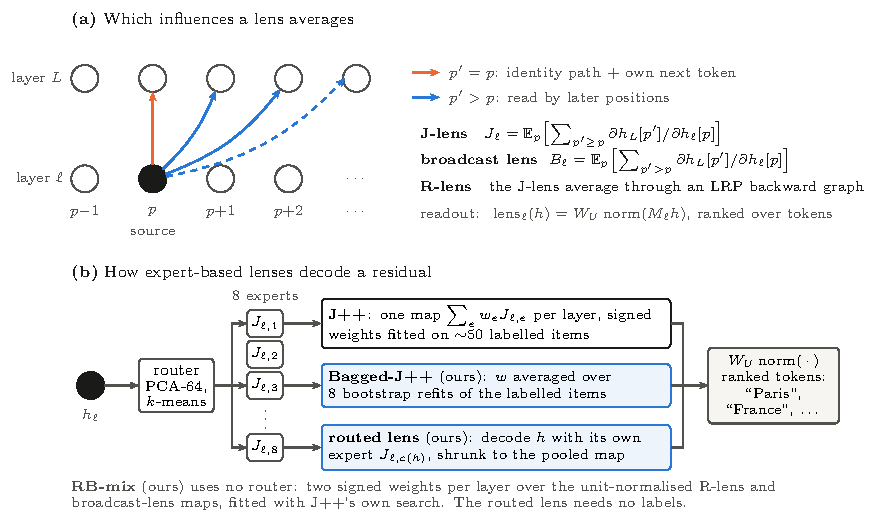
\includegraphics[width=\linewidth]{figures/schematic.pdf}
\caption{The lenses compared. (a) The J-lens averages a residual's influence on the final layer at the
same and all later positions; the broadcast lens keeps only later positions, removing the identity path
and the position's own next-token computation; the R-lens computes the J-lens average through an LRP
backward graph. (b) Expert-based lenses route a residual to one of eight cluster-specific Jacobians. J++
combines them with signed weights fitted on labelled items; Bagged-J++ averages those weights over
bootstrap refits; the routed lens decodes each residual with its own expert and needs no labels.}
\label{fig:schematic}
\end{figure}

% =====================================================================
\section{Background and related work}
\label{sec:background}

\paragraph{The Jacobian lens and J-space.}
Let $h_\ell[p]\in\R^d$ be the residual stream after block $\ell$ at position $p$, and $L$ the last
block. \citet{gurnee2026workspace} define, over pretraining-like text,
\begin{equation}
\label{eq:jlens}
\Jl \;=\; \E_{p}\Big[\sum_{p'\ge p} \frac{\partial h_L[p']}{\partial h_\ell[p]}\Big],
\qquad
\text{lens}_\ell(h) \;=\; W_U\,\mathrm{norm}(\Jl\, h),
\end{equation}
so that a residual is read by what it is disposed to make the model say at the current and all later
positions. The span of the per-token directions $\Jl^{\top} a_t$, where $a_t$ is token $t$'s
unembedding row with the final-norm gain folded in, is the J-space. They argue that J-space content
has functional properties of a global workspace: it is used causally downstream, confined to a
mid-depth band, flexibly routed, selective, and capacity-limited. A reference implementation and
synthetic prompt sets are public.

\paragraph{Improving the J-lens.}
The R-Lens \citep{blank2026rlens} computes the same average through a layer-wise relevance
propagation (LRP) backward graph \citep{bach2015lrp}. The J++ lens \citep{ayonrinde2026jpp} adds
\emph{Jacobian filtering}: source positions are clustered (unit-normalise, PCA to 64 dimensions,
$k$-means with $E=8$ per layer), one expert Jacobian is averaged per cluster, and the experts are
combined with signed weights learned on a labelled fitting split. J++ also uses the LRP backward
pass and \emph{Readout Filtering}, which drops tokens with no letter or digit from the ranking.

\paragraph{Other lenses.}
The logit lens \citep{nostalgebraist2020logitlens} decodes an intermediate residual with the
unembedding directly and is uninformative in early and middle layers. The tuned lens
\citep{belrose2023tuned} learns an affine translator per layer trained on the model's current output,
and so tends to skip ahead to the imminent prediction. Future Lens \citep{pal2023future} and
Patchscopes \citep{ghandeharioun2024patchscopes} decode hidden states by learned or prompted
transplantation.

\paragraph{Randomized estimation.}
Our sketch estimators are instances of classical randomized linear algebra: Hutchinson-style
probing \citep{hutchinson1989}, random-projection sketches \citep{halko2011,martinsson2020}, and
importance sampling for approximate matrix products \citep{drineas2006}, combined with control
variates \citep{owen2013}.

% =====================================================================
\section{Methods}
\label{sec:methods}

All lenses map $h_\ell$ to logits $W_U\,\mathrm{norm}(M_\ell h_\ell)$ for a $d\times d$ map
$M_\ell$: the identity for the logit lens, $\Jl$ for the J-lens, the LRP-graph average for the R-lens,
and a signed combination of expert maps for J++. This section describes what we add.

\subsection{The broadcast lens}
\label{sec:broadcast}

The $p'=p$ term of \cref{eq:jlens} differs in kind from the others. It contains the residual skip
path, which contributes exactly the identity, and the position's own next-token computation. The
terms with $p'>p$ exist only because later positions \emph{read} position $p$ through attention. On a
global-workspace reading, that cross-position traffic is what makes content available: the workspace
is defined by broadcast, not by what a position is about to emit itself. The reference lens shows
the cost of mixing the two: at a sentence-final period, generic sentence openers (``They'', ``The'',
``This'', ``It'') occupy top-10 slots in about a quarter of fitting-split item--layer cells.

\begin{definition}[Broadcast lens]
$B_\ell = \E_p\big[\sum_{p'\in T(p)} \partial h_L[p'] / \partial h_\ell[p]\big]$, where every
$p'\in T(p)$ satisfies $p'>p$.
\end{definition}

The diagonal cannot be removed from a single target-summed backward pass, because one vector--Jacobian
product (VJP) returns each source position's total over all targets. We therefore split each
record's valid positions ($16,\dots,T-2$) into halves, take sources from the first half and place the
one-hot cotangent on every position of the second. Every term then has $p'>p$, the identity path is
absent, and the cost is the same $d$ VJPs per prompt as the reference estimator. The estimator matches
the brute-force Jacobian of a small random Qwen3 model to a relative error of about $10^{-7}$. Lens
logits are invariant to rescaling the map, so the differing number of targets per source does not
matter. The B-lens needs no labels: it is a different definition of the lens, not a fitted correction.

\subsection{Label-free filtering and routed experts}
\label{sec:labelfree}

J++'s expert weights depend on labelled items from the distribution the lens is scored on, a barrier
for a tool meant to read unknown content. We consider two label-free alternatives.

\emph{Future-token weights (SS-J++).} The J-lens measures what a position is disposed to make the model
say later, and on unlabelled text we know what was said later. For 200 held-out WikiText-103
\citep{merity2016wikitext} positions we take as candidates the semantic tokens among
$t_{p+1},\dots,t_{p+16}$ and fit the expert weights with J++'s own search. \emph{Semi-J++} fits on the
union of these rows and the labelled fitting items.

\emph{Routed lens.} J++ collapses its experts into one map per layer, yet the router that defines the
clusters is cheap. The routed lens decodes each residual through the expert of its own cluster,
$W_U\,\mathrm{norm}(J_{\ell,c(h)} h)$, with shrinkage toward the pooled map,
$J_{\ell,e}(\lambda)=\lambda J_{\ell,e}+(1-\lambda)\bar J_\ell$. We consider $\lambda\in\{0.5,1\}$ and
a count-adaptive $\lambda_e=n_e/(n_e+\kappa)$ with $\kappa=200$, where $n_e$ is the number of fitting
positions expert $e$ saw.

\subsection{Candidate improvements to J++}
\label{sec:candidates}

J++ chooses eight signed weights per layer to maximise recall on about 50 labelled items, and fits
them far better than it generalises (\cref{sec:jpp}). We therefore designed candidates that either
stabilise the weight search or feed it better maps. All use J++'s own search (exact recall@10 with a
sigmoid-margin surrogate, three starts, 200 Adam steps) on the same fitting items, over maps scaled to
unit Frobenius norm.

\begin{itemize}
\item \textbf{Bagged-J++} refits the J++ weights on $B=8$ bootstrap resamples of the fitting items,
stratified by evaluation, then averages and renormalises the weight vectors. Averaging reduces the
variance of a search whose objective is a step function of the weights.
\item \textbf{RB-mix} fits two signed weights per layer over the R-lens and the B-lens: two maps that
differ in kind (total influence through the LRP graph; influence on later positions only) rather than
in cluster.
\item \textbf{JppB} first fits J++, then two weights over the J++ map and the B-lens.
\item \textbf{Routed-J++} routes each residual to its own LRP expert, shrunk toward the fitted J++
map with $\lambda_e=n_e/(n_e+200)$.
\item \textbf{RLB-mix} (round 3) is RB-mix with the B-lens computed under the R-Lens's LRP rules.
\end{itemize}
Round 2 fixed the first four candidates, and round 3 fixed RLB-mix, each in a committed
pre-registration before any of its numbers were computed.

\subsection{Sketch estimators of the J-lens}
\label{sec:sketchmethod}

For a prompt $n$ with valid positions $P$, the reference estimator computes
\begin{equation*}
J_n=\frac{1}{|P|}\sum_{p\in P}\sum_{p'\in P}\frac{\partial h_L[p']}{\partial h_\ell[p]}
\end{equation*}
one row at a time: a one-hot cotangent $e_i$ at every target position returns row $i$ at every source position and every
source layer in one VJP. Each prompt costs $d$ VJPs (1,024 here, 5,120 at 27B).

\begin{observation}[Exact identity path]
The $p'=p$ term contains the residual connection, so $J_n=I+\Delta_n$; the identity needs no
estimation.
\end{observation}

\paragraph{Estimator.} Draw a Haar-random $Q\in\R^{d\times K}$ with orthonormal columns, fix a
symmetric positive-definite shaping matrix $W$ and a control variate $J_0$ independent of $(Q,n)$,
compute the $K$ VJPs $G=(WQ)^{\top}J_n$, and set
\begin{equation}
\hat J_n = J_0 + \tfrac{d}{K}\,W^{-1}Q\big(G-(WQ)^{\top}J_0\big).
\end{equation}

\begin{proposition}[Unbiasedness]
$\E[\hat J_n\mid J_0]=\E[J_n]$.
\end{proposition}
\begin{proof}
$\E[QQ^{\top}]=\frac{K}{d}I$ for a Haar $K$-frame, so
$\E[\frac{d}{K}W^{-1}QQ^{\top}W(J_n-J_0)]=J_n-J_0$.
\end{proof}
This holds for any $J_0$ built from earlier prompts and probes, including the running mean of
earlier estimates (an \emph{online} control variate). Unbiasedness says nothing about variance,
however, and \cref{prop:online} shows that the online control variate's variance explodes.

\begin{proposition}[Variance, $W=I$]
\label{prop:var}
For any $M\in\R^{d\times d}$, $\E\|\frac{d}{K}QQ^{\top}M-M\|_F^2=(\frac{d}{K}-1)\|M\|_F^2$. Each prompt
therefore contributes variance $\sigma^2+(\frac{d}{K}-1)\E\|J_n-J_0\|_F^2$, where
$\sigma^2=\E\|J_n-\E J_n\|_F^2$.
\end{proposition}
Without a control variate the sketch pays for the large mean $\|\E J_n\|^2$, and $J_0=I$ removes the
identity exactly. Neither choice beats the exact estimator:

\begin{corollary}[No sketch beats the exact estimator at equal cost]
\label{cor:cost}
With independent prompts and a fixed $J_0$, a budget of $R$ VJP rows buys $R/d$ exact prompts or $R/K$
sketched ones, with variance $\sigma^2 d/R$ and $\frac{d}{R}\big[\sigma^2+(1-\frac{K}{d})\|\E J_n-J_0\|_F^2\big]$
respectively. Their ratio, $1+(1-\frac{K}{d})\|\E J_n-J_0\|_F^2/\sigma^2$, is at least 1.
\end{corollary}
For Qwen3-0.6B with $J_0=I$ the ratio is 2.1, 3.3 and 5.7 at layers 7, 14 and 21 (\cref{sec:sketch}).
Under independent prompts, sketching can only give \emph{anytime} estimates below one exact prompt's
$d$ rows, spread a budget over $d/K$ times as many \emph{distinct} prompts (which helps when nearby
prompts are correlated), and \emph{shape} the probes (\cref{prop:shape}).

\begin{proposition}[The online control variate is unstable]
\label{prop:online}
Let $W=I$, $c=\frac{d}{K}-1$, $J_0=I$ for the first prompt and $J_0=\bar J_n$, the mean of the first $n$
estimates, afterwards. Then $v_n=\E\|\bar J_n-\E J_n\|_F^2$ satisfies
\begin{equation}
v_1=(c+1)\sigma^2+c\|\E J_n-I\|_F^2,\qquad
v_{n+1}=\frac{(n^2+c)\,v_n+(c+1)\sigma^2}{(n+1)^2}.
\end{equation}
\end{proposition}
\begin{proof}
The new estimate's error is $(J_{n+1}-\E J)+(\frac{d}{K}QQ^{\top}-I)(J_{n+1}-\bar J_n)$. Conditional on
the past, both terms have mean zero and are uncorrelated with each other and with $\bar J_n-\E J$.
\Cref{prop:var} gives the second term's variance, $c(\sigma^2+v_n)$. Averaging into the running mean
gives the recursion.
\end{proof}
The coefficient $(n^2+c)/(n+1)^2$ exceeds 1 while $n<(c-1)/2$. Each sketched prompt re-amplifies the
current error of $J_0$ by $c$, and early on the running mean holds too few prompts to dilute it.
The error therefore \emph{grows} for the first $\approx d/2K$ prompts. For $d/K=64$ it grows through
$n=31$, by $1.8\times10^5$ in variance (430 in norm), and only then decays.
\emph{Fix:} shrink the control variate toward the identity, $J_0=I+\lambda_n(\bar J_n-I)$ with
$\lambda_n=n/(n+d/K)$. The coefficient becomes $(n^2+c\lambda_n^2)/(n+1)^2<1$ for every $n$, so the error
never grows, and $J_0$ still converges to the lens. We derived this fix after the online control
variate diverged, so its test is exploratory.

\begin{proposition}[Readout-aware shaping]
\label{prop:shape}
Readouts use only $AJ$, with $A=W_U\,\mathrm{diag}(g)$. For Gaussian probes the leading term of
$\E\|A(\hat J_n-J_n)\|_F^2$ is $K^{-1}\tr(WMM^{\top}W)\,\tr(W^{-1}A^{\top}AW^{-1})$ with $M=J_n-J_0$.
Under an isotropic prior $MM^{\top}\propto I$ it is minimised by $W=(A^{\top}A)^{1/4}$, which reduces
the variance relative to $W=I$ by
\begin{equation}
\rho(A)=\frac{(\sum_i s_i)^2}{d\sum_i s_i^2}\le 1,
\end{equation}
where $s_i$ are the singular values of $A$.
\end{proposition}
\begin{proof}[Proof sketch]
Write $Z=W^2$. By Cauchy--Schwarz for the trace inner product,
$\tr(Z)\tr(Z^{-1}A^{\top}A)\ge(\tr(A^{\top}A)^{1/2})^2$, with equality at $Z\propto(A^{\top}A)^{1/2}$.
\end{proof}
$\rho(A)$ is computed from the weights alone, so it predicts the benefit of shaping before any
Jacobian is computed.

% =====================================================================
\section{Experimental setup}
\label{sec:setup}

\paragraph{Model and hardware.} Qwen3-0.6B (28 blocks, $d=1024$, vocabulary 151,936, tied
embeddings) in bf16 on one 4-core Xeon CPU with AMX and 15\,GB of RAM. Layer $\ell$ means the output of
block $\ell$; the target is block 27 before the final RMSNorm. An exact prompt (1,024 VJPs over 128
tokens) takes 2.5--3 minutes; a $K=16$ sketch prompt about 2.5 seconds.

\paragraph{Fitting data.} WikiText-103 training records of at least 600 characters, truncated to 128
tokens, as in the reference implementation. Exact lenses use records 0--31; sketches use records
0--511. The router and the regression lens use 12,288 positions from records 5000--5255.

\paragraph{Lenses.} The \emph{regression lens} is ridge least squares from $h_\ell$ to $h_{27}$ (held-out
$R^2$ from 0.21 at layer 0 to 0.75 at layer 24), a tuned-lens-style baseline. The \emph{J-lens} and the
\emph{R-lens} use the exact estimator on 32 prompts; the R-lens applies J++'s ``rlens'' LRP rules
(LN rule on residual RMSNorms, identity rule on SiLU, half rule on the gate--up product). J++ follows
the reference code, including the fallback that replaces an expert seen by fewer than 50 positions
with the pooled Jacobian. The \emph{B-lens} uses the first 8 prompts; the J-lens's recall is flat from 8
to 32 prompts (\cref{sec:readout}).

\paragraph{Readout evaluation.} We use the six released prompt sets with their readout positions,
single-token surface forms and min-over-surfaces ranks. Items count only if the model's greedy next
token is correct (multihop, multilingual, order-ops) or matches the rhyme (poetry); association and
typo items are always kept. For Qwen3-0.6B this leaves 14/84 multihop, 15/107 multilingual, 8/98
poetry, 99/99 association and 96/96 typo items, so we also report a pre-declared analysis without the
correctness filter. Recall@$k$ is the fraction of an item's intermediates whose best rank is at most
$k$, averaged over items and then over the five macro evaluations. Intervals are 95\% item bootstraps;
differences use a paired bootstrap.

\paragraph{The J++ protocol.} Head-to-head comparisons follow J++: best rank over seven layers
(4, 7, 11, 14, 18, 21 and 24), Readout Filtering, a stratified 20\%/80\% fitting/held-out split
(47/203 correctness-filtered items), and scores on held-out items only. Every readout choice is made
on the fitting split.

\paragraph{Pre-registration.} Round 2 tests the four candidates of \cref{sec:candidates} on five fresh
splits (seeds 1--5), refitting every label-dependent weight on each split. A candidate beats J++ only
if its mean paired held-out difference is positive \emph{and} it wins on at least four of the five
splits. Held-out sets overlap across splits, so we compute no pooled $p$-value. Round 3 applies the same
rule to 20 further splits (seeds 6--25) with a 16/20 threshold.

\paragraph{Weight-search fidelity.} A line-by-line comparison found that our round-1 port of J++'s
weight search deviated from the reference in three small ways: it masked excluded tokens to $-10^4$
in each expert before combining rather than to $-\infty$ after; it took the surrogate's spread over
non-excluded tokens only; and it broke ties between iterates by order rather than by surrogate value.
Rounds 2 and 3 use a faithful port, about ten times faster, that agreed with full-vocabulary checking
on 960 of 960 steps.

% =====================================================================
\section{Results}

\subsection{Readout recall}
\label{sec:readout}

\Cref{tab:readout} gives recall@10 using the best rank over all 27 block outputs. The J-lens recovers
36.7\% of intermediates against 31.9\% for the logit lens and 16.0\% for the regression lens; with
Readout Filtering the figures are 39.2\% and 33.5\%. The advantage is concentrated in typo
correction (77\% vs 47\%). On multihop and multilingual items the two lenses are indistinguishable at
this sample size.

\begin{table}[t]
\centering
\caption{Recall@10 of latent intermediates (best of layers 0--26, correctness-filtered items). Item
counts in brackets; 95\% item-bootstrap interval on the macro. RF: Readout Filtering.}
\label{tab:readout}
\small
\setlength{\tabcolsep}{3.5pt}
\begin{tabular}{lcccccc}
\toprule
Lens & multihop (14) & multilingual (15) & typo (96) & assoc.\ (99) & poetry (8) & macro \\
\midrule
logit lens & 0.750 & 0.378 & 0.469 & 0.000 & 0.000 & 0.319 [0.265, 0.365] \\
regression lens & 0.250 & 0.311 & 0.240 & 0.000 & 0.000 & 0.160 [0.114, 0.212] \\
J-lens & 0.679 & 0.383 & 0.771 & 0.000 & 0.000 & 0.367 [0.314, 0.418] \\
\addlinespace
logit lens + RF & 0.750 & 0.417 & 0.500 & 0.010 & 0.000 & 0.335 [0.280, 0.383] \\
J-lens + RF & 0.750 & 0.400 & 0.802 & 0.010 & 0.000 & \textbf{0.392} [0.340, 0.441] \\
\bottomrule
\end{tabular}
\end{table}

\begin{figure}[t]
\centering
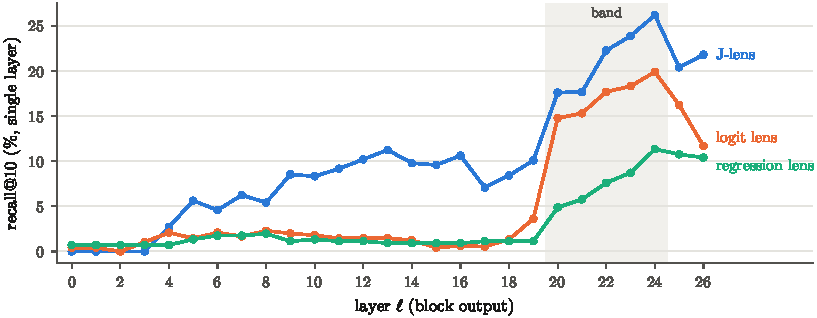
\includegraphics[width=\linewidth]{figures/fig_layers.pdf}
\caption{Single-layer recall@10 by layer. The shaded region is the workspace band selected by the
pre-declared rule (layers 20--24).}
\label{fig:layers}
\end{figure}

\paragraph{The mid-depth picture.} The all-layer maximum hides where the lenses differ
(\cref{fig:layers}). In layers 4--19 the logit lens is near floor (0.4--3.6\% per layer) while the
J-lens recovers 5--11\%. Both peak at layer 24 (26.2\% vs 19.9\%), where they read out the imminent
answer, which is why their best-of-layers scores converge on multihop and multilingual items.

\paragraph{The workspace band.} A rule fixed before any causal experiment takes the contiguous run of
layers around the J-lens peak on which recall stays above half the peak, excluding the three
output-adjacent layers. It selects layers 20--24 (71--86\% of depth), where recall@10 is 23.4\% for
the J-lens against 18.7\% for the logit lens.

\paragraph{Association and poetry are beyond this model.} No lens recovers more than 1\% of
association intermediates or any poetry rhyme plan. The median best rank of the correct association
concept is about 1,000--2,000 for every lens, and of the rhyme about 300--440. All lens differences
below therefore come from multihop, multilingual and typo items.

\paragraph{Fitting budget.} A J-lens fitted on 8 prompts (about 25 CPU-minutes) scores 36.9\% (39.9\%
with RF), the same as on 32. At this size the averaged Jacobian is well determined by a few thousand
source positions.

\subsection{J++ at small scale}
\label{sec:jpp}

\begin{table}[t]
\centering
\caption{Round 1 under the J++ protocol (split seed 0, round-1 port of the weight search). Held-out
macro recall@10 with 95\% interval, paired difference against J++, and held-out recall without the
correctness filter (434 items). $^\dagger$Variant selected on the fitting split within its family.}
\label{tab:round1}
\small
\begin{tabular}{llcccc}
\toprule
Lens & labels & fit split & held out [95\% CI] & $\Delta$ vs J++ [95\% CI] & all items \\
\midrule
logit lens & no & 0.311 & 0.271 [0.206, 0.330] & $-0.104$ [$-0.159$, $-0.048$] & 0.206 \\
regression lens & no & 0.232 & 0.151 [0.100, 0.207] & $-0.223$ [$-0.285$, $-0.167$] & 0.135 \\
J-lens & no & 0.364 & 0.332 [0.266, 0.393] & $-0.042$ [$-0.095$, $+0.012$] & 0.283 \\
R-lens & no & 0.450 & 0.365 [0.302, 0.425] & $-0.010$ [$-0.060$, $+0.042$] & \textbf{0.335} \\
J-filt (plain experts) & yes & 0.483 & 0.354 [0.288, 0.417] & $-0.021$ [$-0.078$, $+0.036$] & 0.297 \\
\textbf{J++} & yes & 0.500 & \textbf{0.374} [0.311, 0.434] & --- & 0.326 \\
\addlinespace
SS-J++ (future tokens) & no & 0.385 & 0.331 [0.269, 0.390] & $-0.043$ [$-0.080$, $+0.002$] & 0.265 \\
Semi-J++ & yes & 0.483 & 0.364 [0.301, 0.423] & $-0.011$ [$-0.029$, $+0.007$] & 0.322 \\
Routed (plain)$^\dagger$ & no & 0.375 & 0.326 [0.262, 0.386] & $-0.049$ [$-0.094$, $-0.013$] & 0.295 \\
Routed-LRP, $\lambda=0.5^\dagger$ & no & 0.450 & 0.369 [0.309, 0.428] & $-0.005$ [$-0.057$, $+0.046$] & --- \\
Routed-LRP, $\kappa=200$ & no & 0.450 & 0.373 [0.312, 0.433] & $-0.001$ [$-0.053$, $+0.050$] & 0.318 \\
B-lens & no & 0.118 & 0.217 [0.157, 0.279] & $-0.157$ [$-0.228$, $-0.085$] & 0.153 \\
JB-mix & yes & 0.364 & 0.368 [0.307, 0.426] & $-0.006$ [$-0.067$, $+0.058$] & 0.291 \\
\bottomrule
\end{tabular}
\end{table}

\Cref{tab:round1} reproduces J++'s head-to-head on one split. J++ reaches 37.4\% held-out recall@10
against 33.2\% for the J-lens, a gain of 4.2 points against about 20 at 27B. Most of it comes from the
LRP backward pass (J-lens $\to$ R-lens, $+3.3$); learned expert weights add $+1.0$ (R-lens $\to$
J++). The weights fit the 47 fitting items far better than they generalise (0.500 against 0.374).
Without the correctness filter the R-lens is the best lens, ahead of J++ by 0.009
[$-0.007$, $+0.026$]. The label-free routed LRP lens matches J++ to within a point; future-token
weights (SS-J++) recover only the J-lens level.

\paragraph{The broadcast lens.} Removing the self-target terms cuts the lens's recall by a third
(0.332 $\to$ 0.217): the identity path carries more information than the generic next-token
predictions it brings with it. Yet the B-lens ranks some intermediates better than every other lens,
for example ``Earth'' (rank 3 against 9--16) and the language name ``Dutch'' (56 against 81--793).

\paragraph{Two pitfalls.} With 32 fitting prompts, one of J++'s eight clusters is empty or nearly so at
each of layers 20--26. Without the reference fallback, an empty cluster gives an all-zero expert map
whose logits all tie, and under the strict rank rule an all-zero map scores a spurious recall of 1.0.
We hit this in a first run and now flag any lens whose fitting-split recall is 1.0. Separately,
masking excluded tokens in each expert before combining penalises negative weight sums; the
reference masks after combining.

\subsection{A pre-registered multi-split test of improvements over J++}
\label{sec:round2}

\begin{table}[t]
\centering
\caption{Round 2 (pre-registered). Confirmatory splits are seeds 1--5; each split refits every
label-dependent weight on 47 items and scores 203. Columns: mean held-out recall@10; mean paired
difference vs J++ with the range over splits; split wins; faithful-port held-out score on the round-1
split (seed 0, not confirmatory). $^\ast$Pre-registered candidate.}
\label{tab:round2}
\small
\begin{tabular}{llcccc}
\toprule
Lens & labels & mean held out & mean $\Delta$ vs J++ [range] & wins & seed 0 \\
\midrule
logit lens & no & 0.285 & $-0.107$ [$-0.127$, $-0.083$] & 0/5 & 0.271 \\
J-lens & no & 0.338 & $-0.055$ [$-0.084$, $-0.036$] & 0/5 & 0.332 \\
R-lens & no & 0.386 & $-0.006$ [$-0.023$, $+0.010$] & 2/5 & 0.365 \\
B-lens & no & 0.210 & $-0.183$ [$-0.204$, $-0.173$] & 0/5 & 0.217 \\
Routed-LRP, $\lambda=0.5$ & no & 0.390 & $-0.002$ [$-0.019$, $+0.014$] & 2/5 & 0.369 \\
Routed-LRP, $\kappa=200$ & no & 0.393 & $+0.000$ [$-0.015$, $+0.014$] & 3/5 & 0.373 \\
\textbf{J++} & yes & 0.392 & --- & --- & 0.367 \\
JB-mix & yes & 0.347 & $-0.045$ [$-0.076$, $-0.026$] & 0/5 & 0.362 \\
\addlinespace
JppB$^\ast$ & yes & 0.396 & $+0.004$ [$-0.017$, $+0.029$] & 3/5 & 0.386 \\
Routed-J++$^\ast$ & yes & 0.380 & $-0.013$ [$-0.034$, $-0.003$] & 0/5 & 0.348 \\
\textbf{RB-mix}$^\ast$ & yes & 0.398 & $\mathbf{+0.006}$ [$+0.000$, $+0.023$] & \textbf{4/5}, 1 tie & 0.395 \\
\textbf{Bagged-J++}$^\ast$ & yes & \textbf{0.403} & $\mathbf{+0.010}$ [$-0.030$, $+0.058$] & \textbf{4/5} & 0.384 \\
\bottomrule
\end{tabular}
\end{table}

\begin{figure}[t]
\centering
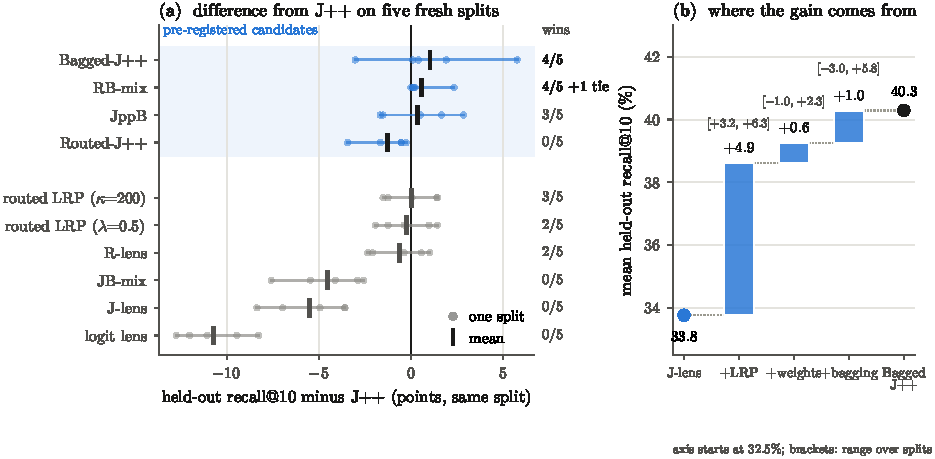
\includegraphics[width=0.68\linewidth]{figures/fig_round2.pdf}
\caption{Round 2: held-out recall@10 minus J++'s on the same split, for each of the five confirmatory
splits (dots), with the mean (bar) and split wins (right; bold where the pre-registered criterion is
met). Shaded rows are the pre-registered candidates.}
\label{fig:round2}
\end{figure}

\paragraph{Two candidates meet the criterion, by small margins.} Bagged-J++ gains 1.0 point on
average and wins on four of five splits; RB-mix gains 0.6 points, wins on four, ties on the fifth and
is never behind J++ (\cref{tab:round2,fig:round2}). JppB ($+0.4$, 3/5) and Routed-J++ ($-1.3$, 0/5)
do not meet the criterion. By the rule fixed in advance, Bagged-J++ and RB-mix beat J++ on this
benchmark; round 3 (\cref{sec:round3}) shows that neither replicates.

\paragraph{The margins are small relative to the noise.} RB-mix's per-split paired 95\% intervals
include zero on every split. Bagged-J++'s exclude zero on two splits but in opposite directions
($+0.058$ [$+0.004$, $+0.124$] on seed 4; $-0.030$ [$-0.069$, $-0.004$] on seed 5). Three of RB-mix's
four wins are below $+0.002$, each the net of gains and losses that nearly cancel. Every split's
held-out set is 80\% of the same 250 items, so four wins in five is weaker evidence than four
independent replications. We read both results as ``at least as good as J++'', not as a clear
improvement.

\paragraph{What bagging changes is overfitting.} Unfitted lenses score lower on the fitting items than
on the held-out items (the R-lens 0.340 against 0.386), so the fitting items happen to be about 4.6
points harder. Against that baseline J++ is optimistic on its fitting items by about 14 points (0.484
against 0.392), Bagged-J++ by about 9 (0.448 against 0.403) and RB-mix, with two weights per layer, by
about 6 (0.416 against 0.398). The candidates that do well give the labelled items the least room to
overfit.

\paragraph{Where RB-mix gains.} RB-mix improves on J++'s multihop recall on four of five confirmatory
splits ($+0.04$ to $+0.17$) and ties on the fifth, while scoring below J++ on multilingual items on
three. The fitted B-lens weight is positive at every layer from 11 onward on average (0.18, 0.33, 0.27,
0.30, 0.49 at layers 11--24) against an R-lens weight of about 0.8--1.0. This matches round 1's
observation that the broadcast lens ranks some bridge entities the other lenses miss.

\paragraph{What does not replicate.} Round 1's JB-mix gain over the J-lens (0.332 $\to$ 0.368) was
mostly a property of that split: over seeds 1--5 JB-mix improves on the J-lens by only 0.010 on average.
The broadcast lens adds to the R-lens but barely to the J-lens.

\paragraph{How much do learned weights add?} Across these five splits J++ improves on the J-lens by
5.5 points (range 3.6--8.4) but on the R-lens by only 0.6 (range $-1.0$ to $+2.3$), which suggested
that almost all of J++'s advantage comes from the LRP backward pass; round 3 revises this. On the round-1
split the faithful port gives J++ 0.367 (0.374 with the round-1 port), which places the label-free
routed LRP lens 0.6 points above it there; over seeds 1--5 the two tie exactly on average.

\subsection{Round 3: the round-2 winners do not replicate}
\label{sec:round3}

Round 2's winners had margins below a single split's paired interval, on five overlapping splits.
Round 3, pre-registered before any of its numbers existed, re-tests Bagged-J++ and RB-mix on twenty
new splits (seeds 6--25), together with RLB-mix (RB-mix with the broadcast lens computed through the
LRP rules). A candidate beats J++ only with a positive mean difference and at least 16 wins in 20. As a
secondary analysis, the fitted lenses are also scored on the 289 items that fail the correctness filter,
which round 2 never scored.

\begin{table}[t]
\centering
\caption{Round 3 (pre-registered; twenty splits of 47 fitting and 203 held-out items). Mean held-out
recall@10, mean paired difference against J++ with the range over splits, wins/ties/losses, and the
mean on the 289 out-of-pool items with its difference against J++. $^\ast$Pre-registered candidate.}
\label{tab:round3}
\small
\setlength{\tabcolsep}{4pt}
\begin{tabular}{llccccc}
\toprule
Lens & labels & mean held out & mean $\Delta$ vs J++ [range] & W/T/L & out of pool & $\Delta$ \\
\midrule
Bagged-J++$^\ast$ & yes & \textbf{0.407} & $+0.003$ [$-0.029$, $+0.054$] & 11/1/8 & 0.223 & $-0.005$ \\
RB-mix$^\ast$ & yes & 0.401 & $-0.004$ [$-0.063$, $+0.035$] & 7/0/13 & 0.223 & $-0.006$ \\
RLB-mix$^\ast$ & yes & 0.400 & $-0.004$ [$-0.072$, $+0.044$] & 9/0/11 & 0.219 & $-0.009$ \\
\textbf{J++} & yes & 0.404 & --- & --- & 0.228 & --- \\
\addlinespace
routed LRP, $\kappa=200$ & no & 0.385 & $-0.019$ [$-0.080$, $+0.033$] & 3/0/17 & 0.201 & $-0.028$ \\
R-lens & no & 0.378 & $-0.026$ [$-0.088$, $+0.027$] & 3/0/17 & \textbf{0.238} & $+0.009$ \\
J-lens & no & 0.334 & $-0.070$ [$-0.127$, $-0.036$] & 0/0/20 & 0.202 & $-0.026$ \\
logit lens & no & 0.275 & $-0.129$ [$-0.187$, $-0.094$] & 0/0/20 & 0.153 & $-0.076$ \\
LRP broadcast lens & no & 0.269 & $-0.135$ [$-0.205$, $-0.089$] & 0/0/20 & 0.117 & $-0.111$ \\
broadcast lens & no & 0.207 & $-0.197$ [$-0.260$, $-0.154$] & 0/0/20 & 0.060 & $-0.168$ \\
\bottomrule
\end{tabular}
\end{table}

\begin{figure}[t]
\centering
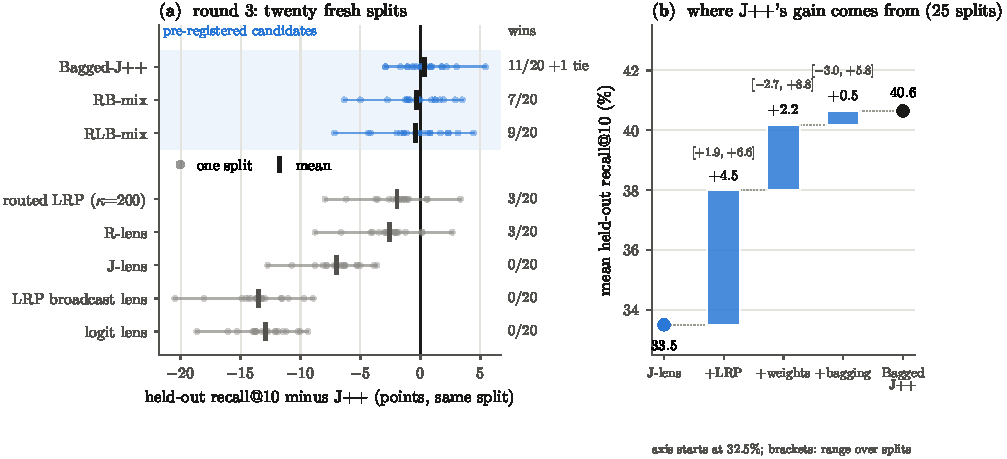
\includegraphics[width=\linewidth]{figures/fig_round3.pdf}
\caption{Round 3. (a) Held-out recall@10 minus J++'s on each of twenty splits (dots), with the mean
(bar) and split wins. (b) Where J++'s gain over the J-lens comes from, as means over all 25 splits of
rounds 2 and 3: the LRP backward pass (J-lens $\to$ R-lens), learned expert weights (R-lens $\to$ J++)
and bagging (J++ $\to$ Bagged-J++); brackets give each step's range over splits.}
\label{fig:round3}
\end{figure}

\paragraph{No candidate beats J++.} Bagged-J++ is ahead by 0.3 points on average and wins 11 of 20
splits; RB-mix and RLB-mix trail by 0.4 and win 7 and 9 (\cref{tab:round3,fig:round3}). None comes near
the 16 wins required. Round 2's small wins were within noise: on this benchmark at 0.6B, nothing we tried
beats J++ under its own protocol.

\paragraph{Bagging curbs overfitting without improving held-out recall.} J++ scores 9.8 points higher
on its fitting items than held out, against 4.0 for Bagged-J++ and RB-mix and about 1 for unfitted
lenses. The weights are less overfitted but generalise no better.

\paragraph{Learned weights add more than round 2 suggested.} Over these twenty splits J++ beats the
R-lens by 2.6 points, on 17 of 20 splits (range $-2.7$ to $+8.8$). Pooled over all 25 splits
(\cref{fig:round3}b), J++'s 6.7-point gain over the J-lens splits into 4.5 points from the LRP backward
pass and 2.2 from the expert weights: LRP is about two-thirds of the gain, not nearly all of it.

\paragraph{The label-free routed lens trails J++.} It tied J++ in round 2 but trails by 1.9 points here
(J++ ahead on 17 of 20); over all 25 splits it trails by 1.6 points. Without labels, a routed LRP lens
gets within two points of J++, not to parity.

\paragraph{LRP helps the broadcast lens, but not in a mix.} The LRP rules raise the broadcast lens from
20.7\% to 26.9\% on all 20 splits, slightly more than they add to the J-lens (4.4 points). Mixed with
the R-lens, the LRP broadcast lens does no better than the plain one.

\paragraph{Out of pool, the plain R-lens is best.} On the 289 items the model answers wrongly, the
R-lens beats J++ by 0.9 points on 15 of 20 splits, and every candidate trails J++ slightly, matching the
round-1 all-items panel. Where the model has not computed the answer, weights tuned on correctly
answered items do not help.

\subsection{Causal use of J-lens directions}
\label{sec:swaps}

\paragraph{Protocol.} Following the reference clamp swap, at every layer of a band and every position
after the first we take the unit lens directions $u_s,u_t$ of a source and a target token (for the
J-lens $\Jl^{\top}a_t$; for the logit lens $a_t$), re-express the residual in the plane they span, and
exchange the two coefficients multiplied by a scale factor. We report the relative change of the
final-position residual (the edit norm). Each trial is run with J-lens, logit-lens and regression-lens
directions, and with an unrelated-noun target as a null. Only trials whose unedited answer is correct
are scored; a trial succeeds when the swapped answer becomes the model's top word. Flexible
generalisation uses templates $f(A)$ (``The capital of A is the city of'') over four categories with
four functions each, swapping $A$ for $B$; success means $f(B)$. The model answers 60 of 170 such
prompts correctly. Two bands were queued before either produced a result: the readout-selected band
(20--24) and the mid-depth layers where the J-lens's readout advantage lies (7--20).

\begin{table}[t]
\centering
\caption{Flexible-generalisation swap success (60 scored trials). Edit norm in brackets. The last
column counts discordant trials (J-lens only / logit lens only).}
\label{tab:swaps}
\small
\begin{tabular}{llcccccc}
\toprule
Band & scale & J-lens & logit lens & regression & J $-$ logit [95\% CI] & disc. \\
\midrule
\multirow{4}{*}{20--24} & 0.5 & 0.117 (0.18) & 0.050 (0.12) & 0.050 (0.16) & $+0.067$ [$+0.017$, $+0.133$] & 4/0 \\
 & 1 & \textbf{0.283} (0.19) & 0.067 (0.14) & 0.150 (0.17) & $+0.217$ [$+0.117$, $+0.317$] & 13/0 \\
 & 2 & 0.283 (0.35) & 0.167 (0.25) & 0.250 (0.31) & $+0.117$ [$+0.017$, $+0.217$] & 9/2 \\
 & 4 & 0.167 (0.79) & 0.183 (0.49) & 0.150 (0.69) & $-0.017$ [$-0.067$, $+0.033$] & 1/2 \\
\addlinespace
\multirow{3}{*}{7--20} & 1 & \textbf{0.483} (0.13) & 0.083 (0.08) & --- & $+0.400$ [$+0.267$, $+0.533$] & 25/1 \\
 & 2 & 0.417 (0.25) & 0.200 (0.14) & --- & $+0.217$ [$+0.083$, $+0.350$] & 17/4 \\
 & 4 & 0.017 (0.54) & 0.217 (0.28) & --- & $-0.200$ [$-0.317$, $-0.100$] & 1/13 \\
\bottomrule
\end{tabular}
\end{table}

\begin{figure}[t]
\centering
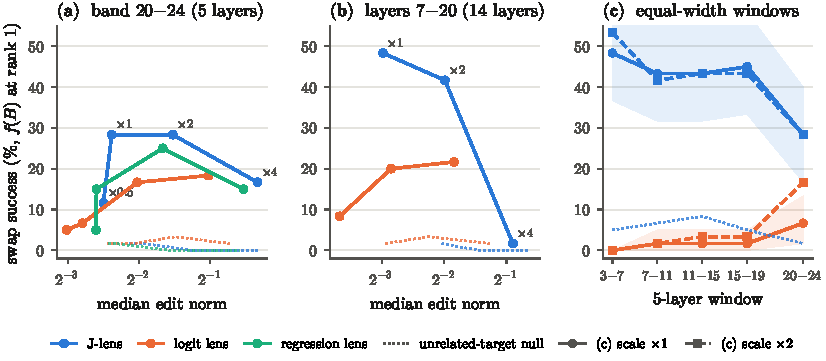
\includegraphics[width=\linewidth]{figures/fig_swaps.pdf}
\caption{Causal swaps (flexible generalisation, 60 scored trials). (a, b) Success against the median
edit norm for each lens and scale (labels) in the two pre-planned bands. (c) Success in equal-width
5-layer windows (exploratory); shaded areas are 95\% intervals at scale 1. Dotted lines are the
unrelated-target nulls.}
\label{fig:swaps}
\end{figure}

\paragraph{J-lens directions are the most efficient handle on the argument.} At scale 1 in the
workspace band, a swap along J-lens directions installs $f(B)$ on 28\% of trials, against 7\% for
logit-lens and 15\% for regression-lens directions, and every discordant trial favours the J-lens
(\cref{tab:swaps}). The advantage survives matching edit norms: the logit lens at scale 2 makes a
larger edit (0.25 against 0.19) and still reaches only 17\% (\cref{fig:swaps}). The unrelated-target
null succeeds on at most one trial in 56--57 at any scale, for any lens.

\paragraph{The leverage is not confined to the readout band.} Across layers 7--20, J-lens swaps succeed
on 48\% of trials against 8\% for the logit lens, with a smaller edit norm than in the late band. In
those layers the logit lens reads out almost nothing (\cref{sec:readout}), yet J-lens directions there
are the most effective handles we found. Larger edits break the computation: at scale 4 the J-lens edit
across 14 layers succeeds on 1 of 60 trials.

\paragraph{Depth, not the number of edited layers (exploratory).} The two pre-planned bands differ in
width, so after seeing them we added four equal-width 5-layer windows on the same 60 trials
(\cref{tab:windows}, \cref{fig:swaps}c). Every window from layer 3 to 19 beats the readout band: J-lens
swaps succeed on 43--48\% of trials there against 28\% in layers 20--24, with edits half the size or
less. On paired trials, layers 15--19 beat layers 20--24 by $+0.167$ [$+0.050$, $+0.283$] (12 trials
only in the window, 2 only in the band). The logit lens moves almost nothing before layer 20 (0--2\%).
The unrelated-target null is higher in the early windows (4--9\%), so the specific effect there is
about 35--45 points, and countries again carry it (24--27 of 36 per window). The J-lens direction of a
function's argument is thus an effective causal handle from layer 3 to layer 19, and becomes less
effective exactly where readouts peak and the logit lens starts to read out the answer. This fits the
function having largely been applied by layers 20--24, so that swapping its argument there comes too
late.

\begin{table}[t]
\centering
\caption{Equal-width windows (exploratory): flexible-generalisation swap success at scale 1 on the same
60 trials. Discordant: trials only the J-lens / only the logit lens gets right.}
\label{tab:windows}
\small
\begin{tabular}{lccccc}
\toprule
Window & J-lens & logit lens & J $-$ logit [95\% CI] (disc.) & null (J-lens) & J edit norm \\
\midrule
layers 3--7 & \textbf{0.483} & 0.000 & $+0.483$ [$+0.350$, $+0.600$] (29/0) & 0.064 & 0.08 \\
layers 7--11 & 0.433 & 0.017 & $+0.417$ [$+0.300$, $+0.533$] (25/0) & 0.042 & 0.10 \\
layers 11--15 & 0.433 & 0.017 & $+0.417$ [$+0.300$, $+0.533$] (25/0) & 0.088 & 0.08 \\
layers 15--19 & 0.450 & 0.017 & $+0.433$ [$+0.316$, $+0.550$] (26/0) & 0.036 & 0.06 \\
layers 20--24 (band) & 0.283 & 0.067 & $+0.217$ [$+0.117$, $+0.317$] (13/0) & 0.018 & 0.19 \\
\bottomrule
\end{tabular}
\end{table}

\paragraph{One category carries the effect.} At scale 1, countries succeed on 16/36 trials (layers
20--24) and 27/36 (layers 7--20) with J-lens directions. Number words (0/15) are not moved by any lens,
and animal attributes only twice. Probe-swap two-hop prompts are uninformative at this scale: the
model answers only 8 of 83 correctly.

\subsection{Ignition}
\label{sec:ignition}

\paragraph{Protocol.} For a concept pair $(A,B)$ in a carrier sentence, the slot token's input
embedding is replaced by $\alpha e_A+(1-\alpha)e_B$ for 21 values of $\alpha\in[0,1]$. At the slot
position and every second layer we read A's reciprocal-rank share
$s=r_A^{-1}/(r_A^{-1}+r_B^{-1})$ and measure the 10\%$\to$90\% transition width in $\alpha$ of the
monotone-smoothed curve. A workspace-like ignition predicts narrow transitions in the band. We run 66
country pairs in 10 carriers (660 trials), and 12 associated noun pairs (e.g.\ bread/butter) and 12
unrelated noun pairs (e.g.\ bread/chips) in 5 carriers each.

\paragraph{Control.} A narrow width alone does not show that the network sharpens anything, because
the reciprocal-rank share is itself non-linear in the logits; a reference width of 0.8 for a linear mix,
which we first used, is not a valid baseline. The control runs only $\alpha=0$ and $\alpha=1$,
interpolates the two residuals in a straight line at each layer, and reads them with the same lens. It
keeps the readout's non-linearity and none of the network's. The actual run and the control agree at
the endpoints (mean absolute share difference 0.0004). \emph{Network sharpening} is the actual width
minus the control width per trial; intervals are cluster bootstraps over concept pairs.

\begin{table}[t]
\centering
\caption{Ignition. Top: median transition width for country pairs, actual and under the linear
control. Bottom: network sharpening for the J-lens (actual $-$ control; negative is sharper), median of
per-trial differences with 95\% intervals clustered by pair.}
\label{tab:ignition}
\small
\setlength{\tabcolsep}{2.6pt}
\begin{tabular}{lcccccccc}
\toprule
Layer & 0 & 8 & 12 & 16 & 20 & 22 & 24 & 27 \\
\midrule
J-lens, actual & 0.33 & 0.32 & 0.27 & 0.25 & 0.17 & 0.12 & 0.11 & 0.19 \\
J-lens, control & 0.32 & 0.40 & 0.41 & 0.39 & 0.34 & 0.26 & 0.27 & 0.52 \\
logit lens, actual & 0.53 & 0.52 & 0.49 & 0.56 & 0.28 & 0.18 & 0.18 & 0.19 \\
logit lens, control & 0.47 & 0.59 & 0.65 & 0.70 & 0.53 & 0.45 & 0.45 & 0.52 \\
\midrule
countries (660) & $-0.00$ & $-0.07$ & $-0.13$ & $-0.12$ & $-0.15$ & $-0.14$ & $-0.16$ & $-0.31$ \\
 & & {\scriptsize[$-.08$,$-.07$]} & {\scriptsize[$-.14$,$-.12$]} & {\scriptsize[$-.14$,$-.11$]} & {\scriptsize[$-.16$,$-.14$]} & {\scriptsize[$-.15$,$-.13$]} & {\scriptsize[$-.16$,$-.15$]} & {\scriptsize[$-.32$,$-.29$]} \\
unrelated nouns (60) & $-0.01$ & $-0.05$ & $-0.04$ & $-0.05$ & $-0.07$ & $-0.08$ & $-0.09$ & $-0.19$ \\
 & & {\scriptsize[$-.09$,$-.02$]} & {\scriptsize[$-.06$,$-.03$]} & {\scriptsize[$-.07$,$-.02$]} & {\scriptsize[$-.08$,$-.06$]} & {\scriptsize[$-.10$,$-.05$]} & {\scriptsize[$-.12$,$-.08$]} & {\scriptsize[$-.22$,$-.16$]} \\
associated nouns (60) & $-0.00$ & $-0.02$ & $-0.02$ & $-0.02$ & $-0.04$ & $-0.09$ & $-0.10$ & $-0.23$ \\
 & & {\scriptsize[$-.04$,$-.01$]} & {\scriptsize[$-.04$,$+.00$]} & {\scriptsize[$-.03$,$-.00$]} & {\scriptsize[$-.06$,$-.01$]} & {\scriptsize[$-.14$,$-.02$]} & {\scriptsize[$-.15$,$-.02$]} & {\scriptsize[$-.32$,$+.14$]} \\
\bottomrule
\end{tabular}
\end{table}

\begin{figure}[t]
\centering
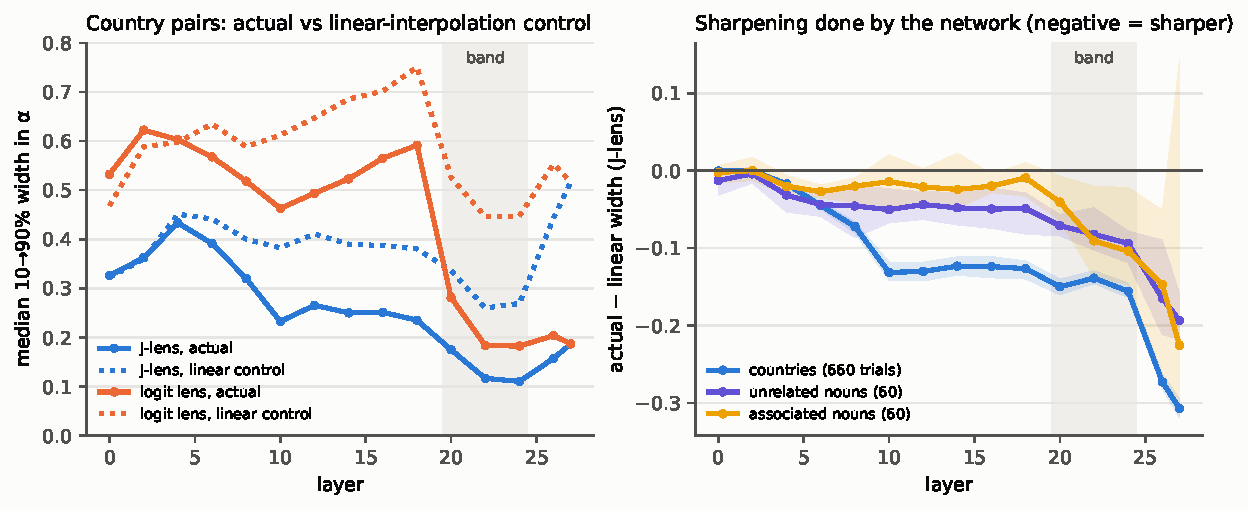
\includegraphics[width=\linewidth]{figures/fig_ignition.pdf}
\caption{Ignition. Left: transition widths for country pairs, actual (solid) and under the
linear-interpolation control (dotted). Right: network sharpening (actual $-$ control) for the J-lens by
pair type, with 95\% intervals clustered by pair. The shaded region is the workspace band.}
\label{fig:ignition}
\end{figure}

\paragraph{The network sharpens the switch, most for countries.} From layer 8 onward the transition
between two countries is narrower than a straight-line mix of the endpoint residuals predicts: by 0.07
at layer 8 and by 0.12--0.16 through layers 12--24 (\cref{tab:ignition,fig:ignition}). Unrelated nouns
sharpen by only about 0.05, and associated pairs such as bread/butter by about 0.02 before layer 20.
Associated concepts evidently co-activate rather than compete, while two countries compete for the
same slot.

\paragraph{But not in a band, and not only through the J-lens.} The sharpening grows steadily to the
output, reaching 0.31 at the final layer, with no peak in layers 20--24. Read through the logit lens,
the network sharpens the country switch as much or more (0.22--0.25 at layers 20--24). The J-lens's
narrower widths are mostly a property of the readout: under the control they are already 0.19--0.31
below the logit lens's in layers 8--16. At 0.6B, the model turns a gradual input mix into an
increasingly categorical choice between competing concepts, the behaviour ignition describes, but it
does so progressively through depth in the residual stream itself rather than as an abrupt event
confined to a J-space band.

\subsection{Sketch estimators}
\label{sec:sketch}

\pending{Learning curves of the sketch estimators (online control variate, shaped probes, identity
control variate, no control variate) against the exact estimator at equal numbers of backward passes,
and the measured gain from shaping against the predicted $\rho(A)$.}

% =====================================================================
\section{Negative results}
\label{sec:negative}

We report three readout modifications we expected to help. On the fitting split two hurt and one made
no difference.

\paragraph{Per-token calibration.} Ranking tokens by the z-score or centred value of their lens logit
relative to corpus statistics lowered all-layer recall@10 of the 8-prompt J-lens from 0.369 to 0.281
(centred) and 0.267 (z-scored), and the logit lens from 0.319 to 0.280. The context-independent prior
that calibration removes carries signal: many latent intermediates are frequent, generic words.

\paragraph{Affine Taylor transport.} Expanding around the corpus mean, $\mu_L+J(h-\mu_\ell)$, instead
of around zero lowered recall@10 from 0.343 to 0.280 (all items: 0.247 to 0.163). At layer 14,
$\|\mu_L\|=459$ against $\|J\mu_\ell\|=119$, so the true final-layer mean over-weights the generic
output direction.

\paragraph{Surface-form collapsing.} Top-10 lists often spend several slots on one word. Collapsing
tokens that agree after dropping a leading space and lowercasing (37,912 tokens in multi-member
classes) left fitting-split recall unchanged (J-lens 0.364, logit lens 0.311): the duplicated variants
are almost always variants of the correct concept.

% =====================================================================
\section{Discussion}
\label{sec:discussion}

\paragraph{What transfers to 0.6B.} The J-lens is a better reader than the logit lens and a
current-output regression lens, and its directions are causally effective handles on a function's
argument, far above controls. These are the properties most directly tied to the J-lens's definition:
it transports a residual to what the model is disposed to say, and a direction that changes that
disposition changes the answer.

\paragraph{What does not, or not yet.} The large-model picture places workspace content in a
contiguous late band. At 0.6B the readout-selected band (20--24) is where readouts peak, but causal
leverage is larger in every 5-layer window from layer 3 to 19, where readouts are weak, and drops in
the band itself. Implicit concepts (association,
poetry plans) are not recoverable by any linear readout. Ignition-like sharpening is real but grows
steadily to the output and is as visible through the logit lens, so it does not single out a band. We read these as weak evidence against a narrow late
workspace in a 0.6B model, not as evidence against the J-space hypothesis at scale.

\paragraph{What J++ adds at small scale.} About two-thirds of J++'s advantage over the J-lens comes
from the LRP backward pass and a third from its learned expert weights. The weights fit 47 labelled
items far better than they generalise, yet nothing we tried improves on them: stabilising the search
(bagging, two-weight mixes) halves the overfitting without raising held-out recall, and making it richer
(Routed-J++) loses on every split. A label-free routed LRP lens comes within two points. The lesson we
draw is methodological as much as substantive: round 2's five overlapping splits produced two
``wins'' that twenty more splits erased.

\section{Limitations}
\label{sec:limitations}

All results are for one 0.6B model. Small models answer few released items correctly (8--15 each on
multihop, multilingual and poetry), so per-evaluation estimates are noisy; we mitigate this with an
all-items analysis and item-level intervals but cannot separate ``the lens fails'' from ``the model
never computed the intermediate''. Our lenses average 32 prompts against 1,000 for the released
lenses; J++'s experts each see about one eighth of the positions and are the most budget-sensitive
component, so conclusions about J++ at full budget should not be drawn from our numbers. We could not
access the J-space paper's text from our compute environment; our implementation follows the released
code line by line where possible, and choices not pinned down by released code (the seven-layer subset,
the band rule, the ignition statistic, the final-norm gain in J-lens directions) are stated explicitly.
Rounds 2 and 3 vary the split (26 seeds) but not the fitting prompts, the router's $k$-means or the
probe draws, and all splits draw on the same 250 items; the out-of-pool items are a different
population, not a replication on new items. Finally, we test operational consequences and make no claim about consciousness.

\section{Conclusion}

On a 0.6B model, the Jacobian lens reproduces as a better reader and a better causal handle than the
logit lens, but the clean late-band workspace of large models does not: causal leverage is strongest
through mid-depth. J++'s gain shrinks to about 7 points, two-thirds of it from its LRP backward pass;
two pre-registered rounds found nothing that beats it, and a label-free routed lens comes within two
points. The network sharpens competing concepts into a categorical choice, but
progressively through depth rather than in a band. \pending{Sketch estimator results.}

\section*{Reproducibility}
Code, results, logs, pre-registrations and the exact commands are in the project repository
(\url{https://github.com/d4solxt3/basic-mnist-classifier}, branch
\texttt{claude/\allowbreak jspace-qwen-\allowbreak reproduction-\allowbreak hbhcoo}, folder \texttt{jspace-qwen}). Appendix~\ref{app:repro}
lists the pipeline.

\bibliographystyle{plainnat}
\bibliography{refs}

\clearpage
\appendix

\section{Reproduction pipeline}
\label{app:repro}

End to end the pipeline takes about 11 CPU-hours on 4 cores. Each step writes a JSON file under
\texttt{results/}.

\begin{center}
\small
\begin{tabular}{p{0.32\linewidth}p{0.42\linewidth}r}
\toprule
Step & Script (results file) & Time \\
\midrule
Estimator correctness & \texttt{test\_estimators.py} & 1 min \\
Corpus data, router, future targets & \texttt{collect.py}, \texttt{routing.fit\_router}, \texttt{collect\_future.py} & minutes \\
J-lens, R-lens (32 prompts each) & \texttt{fit.py --method exact [--lrp]} & 80 min each \\
B-lens (8 prompts) & \texttt{fit.py --targets later} & 21 min \\
Readouts and band & \texttt{readout\_eval.py}, \texttt{choose\_band.py} (\texttt{readout\_main.json}, \texttt{band.json}) & minutes \\
J++ round 1 & \texttt{jpp\_compare.py} (\texttt{jpp\_compare\_main*.json}) & 1--1.5 h \\
J++ round 2 & \texttt{jpp\_splits.py} (\texttt{jpp\_splits\_round2.json}) & 35 min \\
Swaps & \texttt{swaps.py}, \texttt{swap\_stats.py} (\texttt{swaps\_*.json}, \texttt{swap\_stats.json}) & 15 min \\
Swap windows (exploratory) & \texttt{run\_windows.sh} (\texttt{swaps\_win*.json}) & 20 min \\
Ignition and control & \texttt{ignition.py}, \texttt{ignition\_stats.py} (\texttt{ignition\_main*.json}) & 20 min per run \\
Round 3 & \texttt{fit.py --targets later --lrp}, \texttt{jpp\_splits.py} (\texttt{jpp\_splits\_round3.json}) & 2 h \\
Sketch estimators & \texttt{fit.py --method sketch}, \texttt{curves.py} (\texttt{curves.json}) & 1.5 h \\
Shaping predictor $\rho(A)$ & \texttt{rho.py} (\texttt{rho.json}) & 1 min \\
Figures & \texttt{figures.py}; \texttt{figures/schematic.tex} & 1 min \\
\bottomrule
\end{tabular}
\end{center}

\section{Pre-registrations}
\label{app:prereg}

Both pre-registrations were committed to the repository before any of their numbers were computed
(\texttt{paper/prereg\_round2.md}, \texttt{paper/prereg\_round3.md}). Round 2 records one amendment,
also made before any round-2 number existed: the switch to the faithful weight-search port. Smoke
tests of the code paths used one layer, a few Adam steps and stand-in maps; their numbers were
discarded.

\end{document}
